\documentclass{beamer}

\usetheme{Madrid}

\usepackage[utf8]{inputenc}
\usepackage[T1]{fontenc}
\usepackage{amsmath}
\usepackage{amsfonts}
\usepackage{amssymb}
\usepackage{tikz}
\usetikzlibrary{quantikz}
\usepackage{lineno}
\usepackage{multirow}

\usepackage{algorithm} % write pseudocode, suggested by IEEEtran instead of algorithm2e
\usepackage{algpseudocode}

\providecommand{\floor}[1]{\left \lfloor #1 \right \rfloor }

\title{Quantum Computing and Cryptography}
\author{Damien, Théo, Matthieu}
\institute{}
\date{February 12, 2025}

\begin{document}

\begin{frame}
\maketitle
\end{frame}

\begin{frame}{Outline}
\tableofcontents
\end{frame}

\section{Intro}
\begin{frame}
  \frametitle{Outline}
  \tableofcontents[currentsection]
\end{frame}

\begin{frame}{Introduction}
\begin{linenumbers}
	\begin{block}<+->{What is Cryptology?}
		\begin{itemize}
			\item Science of secret ($\kappa\rho\nu\pi\tau o\varsigma$) % $\kappa\rho$\u{$\nu$}$\pi\tau\text{\'{o}}\varsigma$ % (κρῠπτός)
			\item Two complementary parts: cryptography and cryptanalysis
		\end{itemize}
	\end{block}
	\begin{block}<+->{Historically}
		\begin{itemize}
			\item Cryptography: hide the content of a message
			\item Cryptanalysis: get the content of this message
		\end{itemize}
	\end{block}
	\begin{block}<+->{Nowadays}
		\begin{itemize}
			\item Cryptography: Create protocols to protect a communication
			\item Cryptanalysis: Measure the security level of those protocols
		\end{itemize}
	\end{block}
\end{linenumbers}
\end{frame}

\section{RSA}
\begin{frame}
  \frametitle{Outline}
  \tableofcontents[currentsection]
\end{frame}

\begin{frame}{RSA}
    \centering
    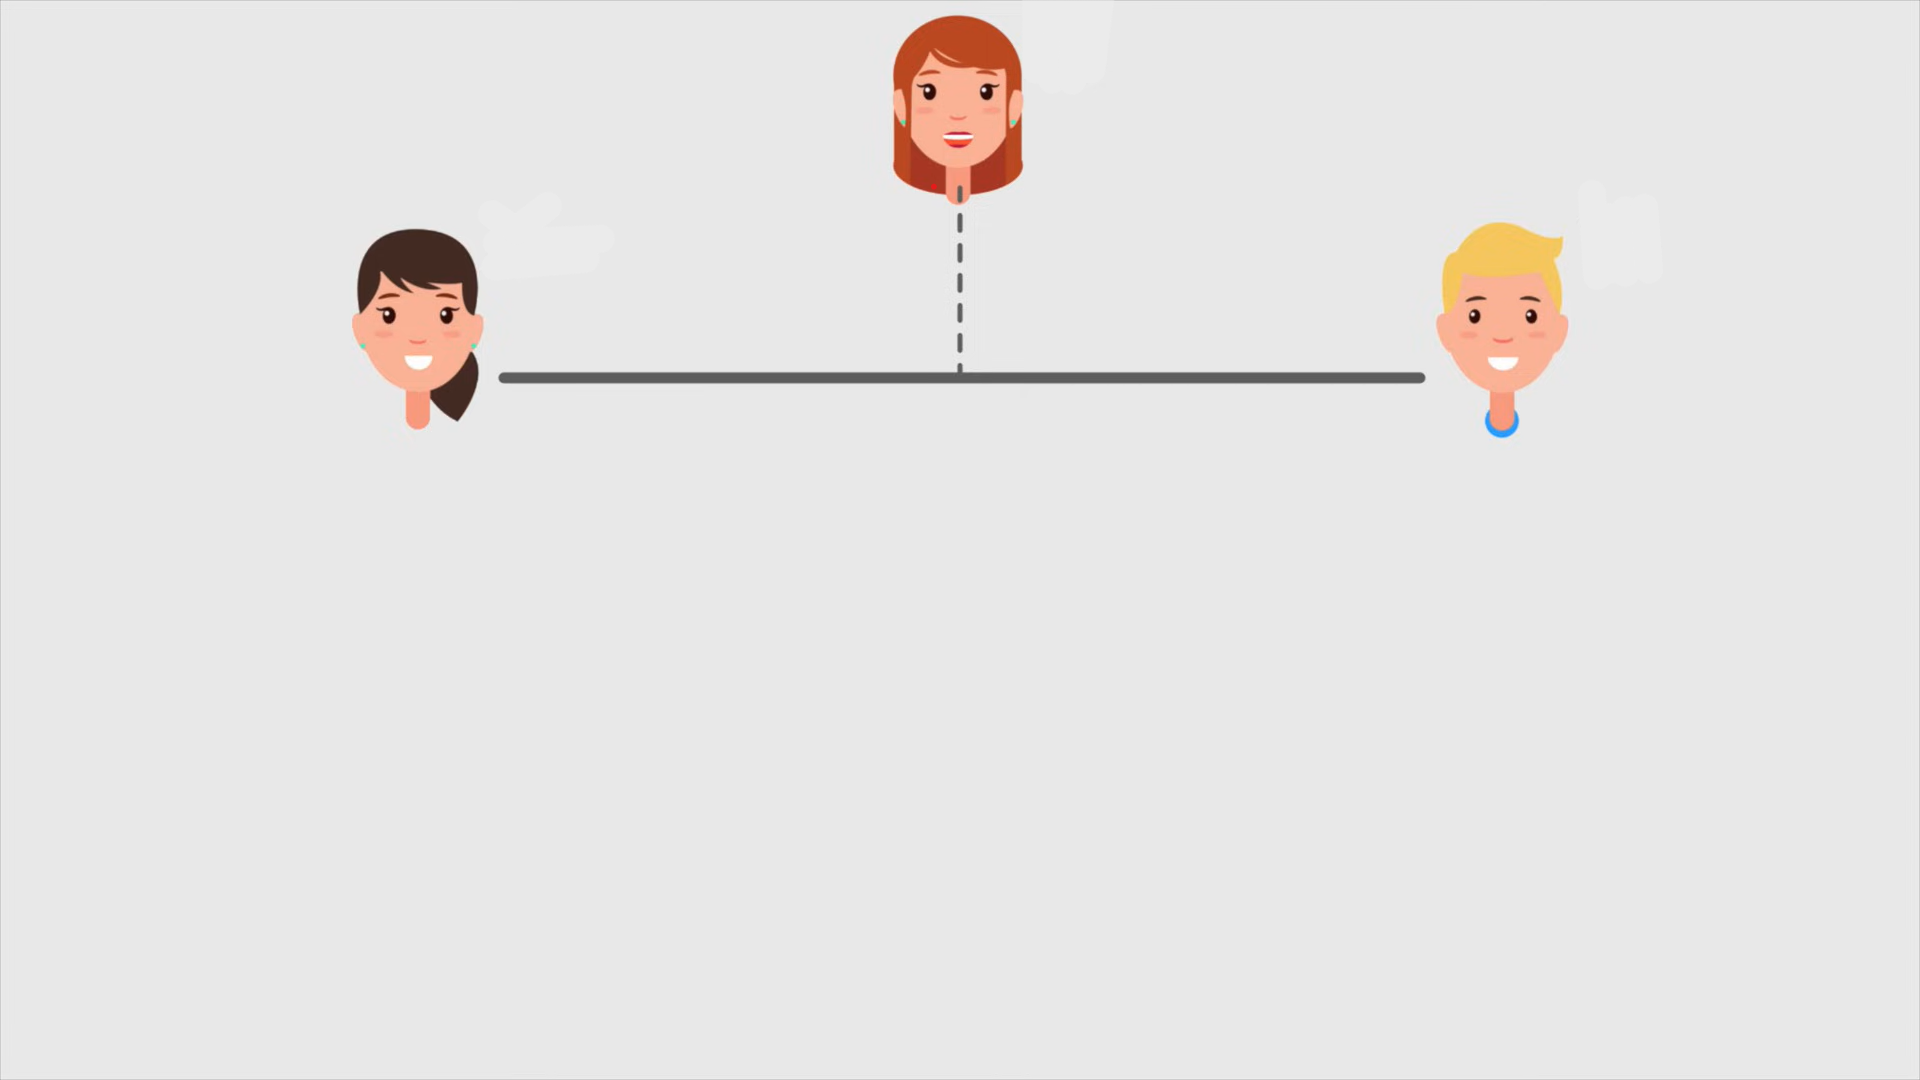
\includegraphics[width=\textwidth, height=0.9\textheight, keepaspectratio]{rsa 1.png}
\end{frame}

\begin{frame}{RSA}
    \centering
    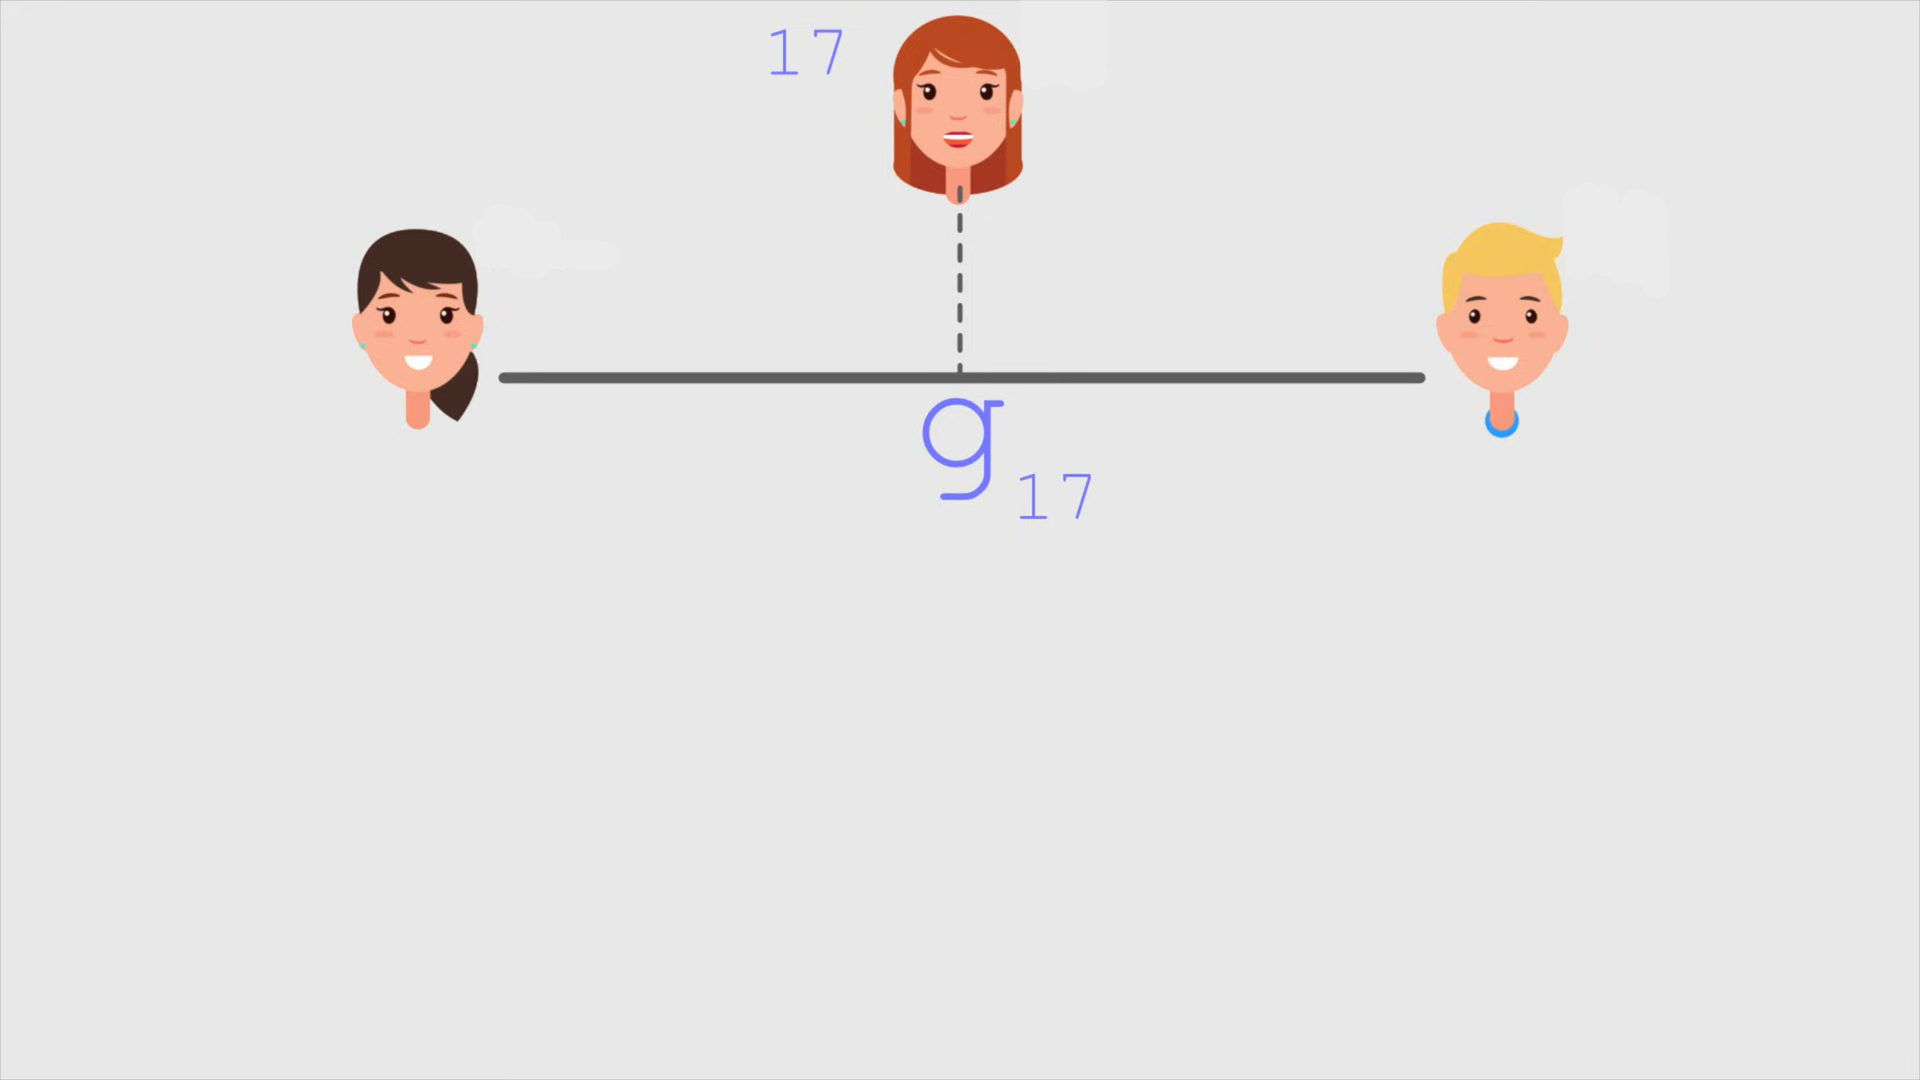
\includegraphics[width=\textwidth, height=0.9\textheight, keepaspectratio]{rsa 2.png}
\end{frame}

\begin{frame}{RSA}
    \centering
    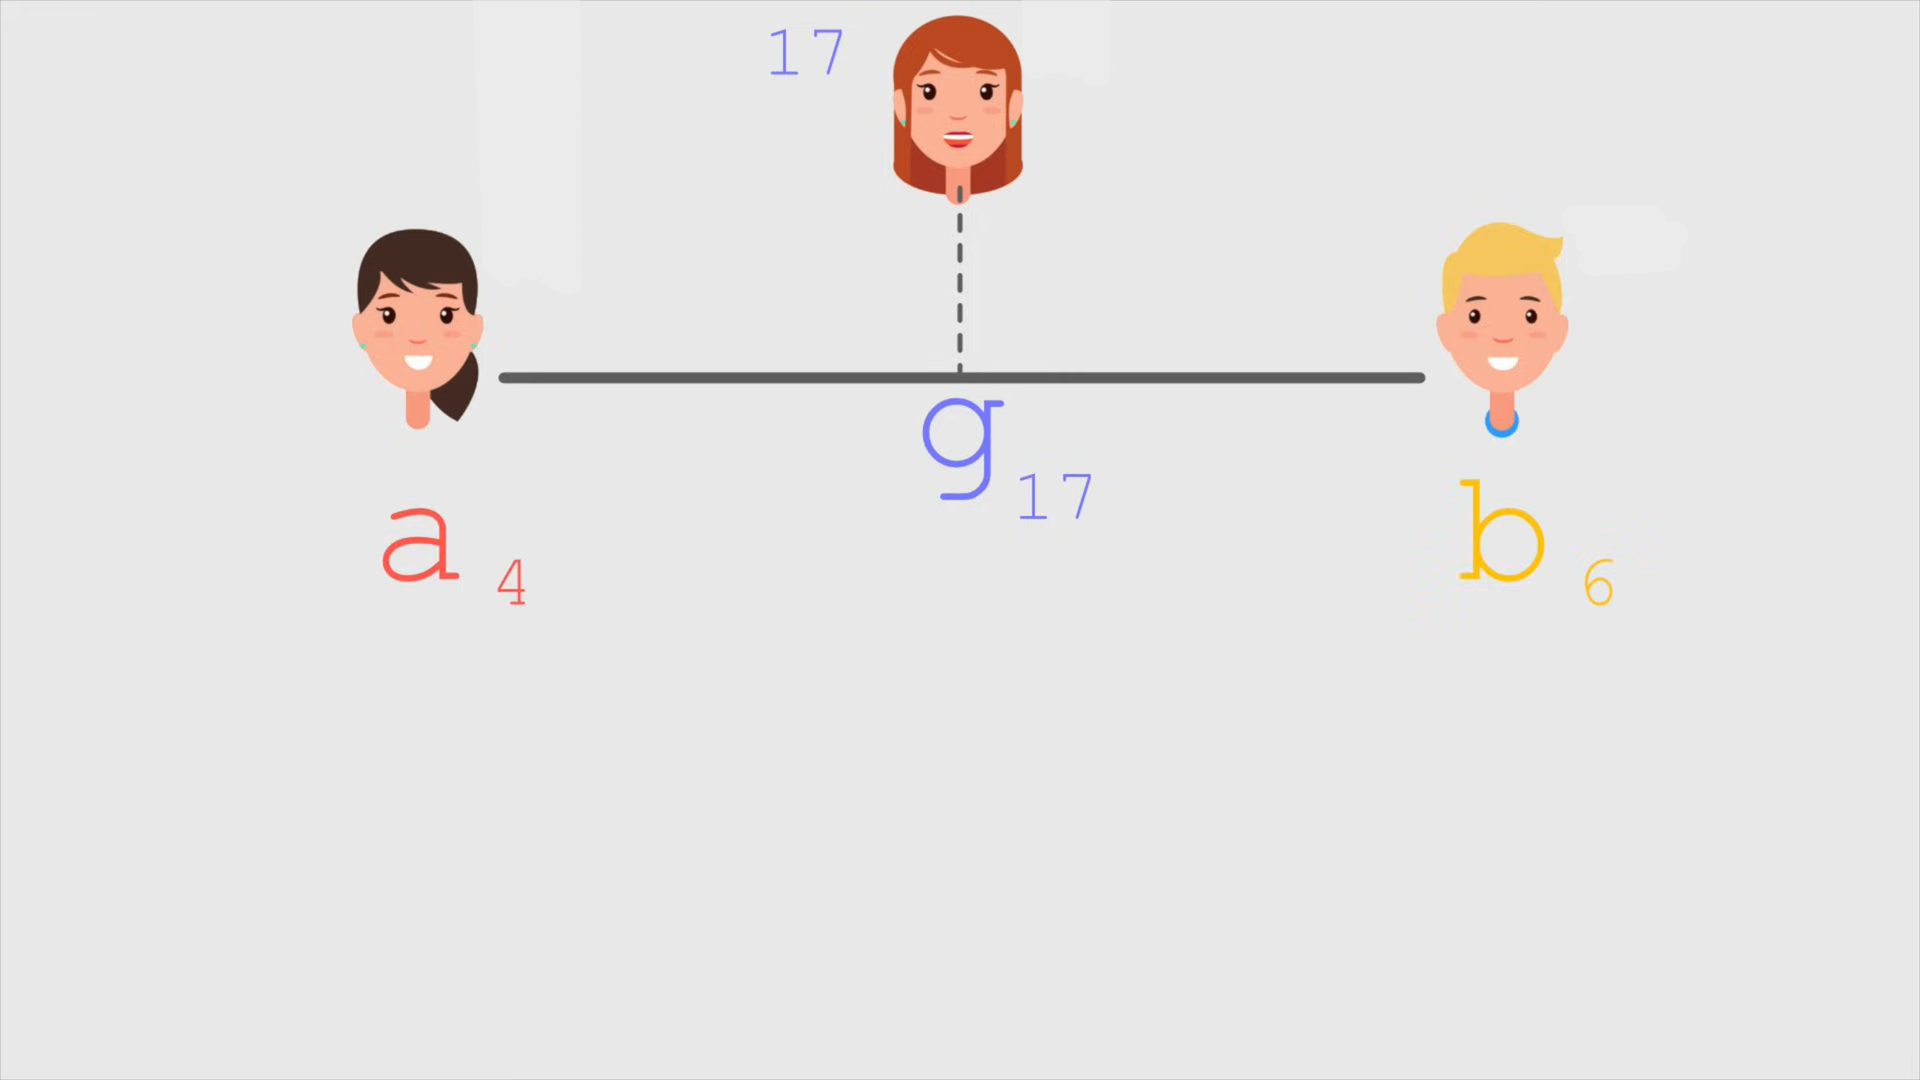
\includegraphics[width=\textwidth, height=0.9\textheight, keepaspectratio]{rsa 3.png}
\end{frame}

\begin{frame}{RSA}
    \centering
    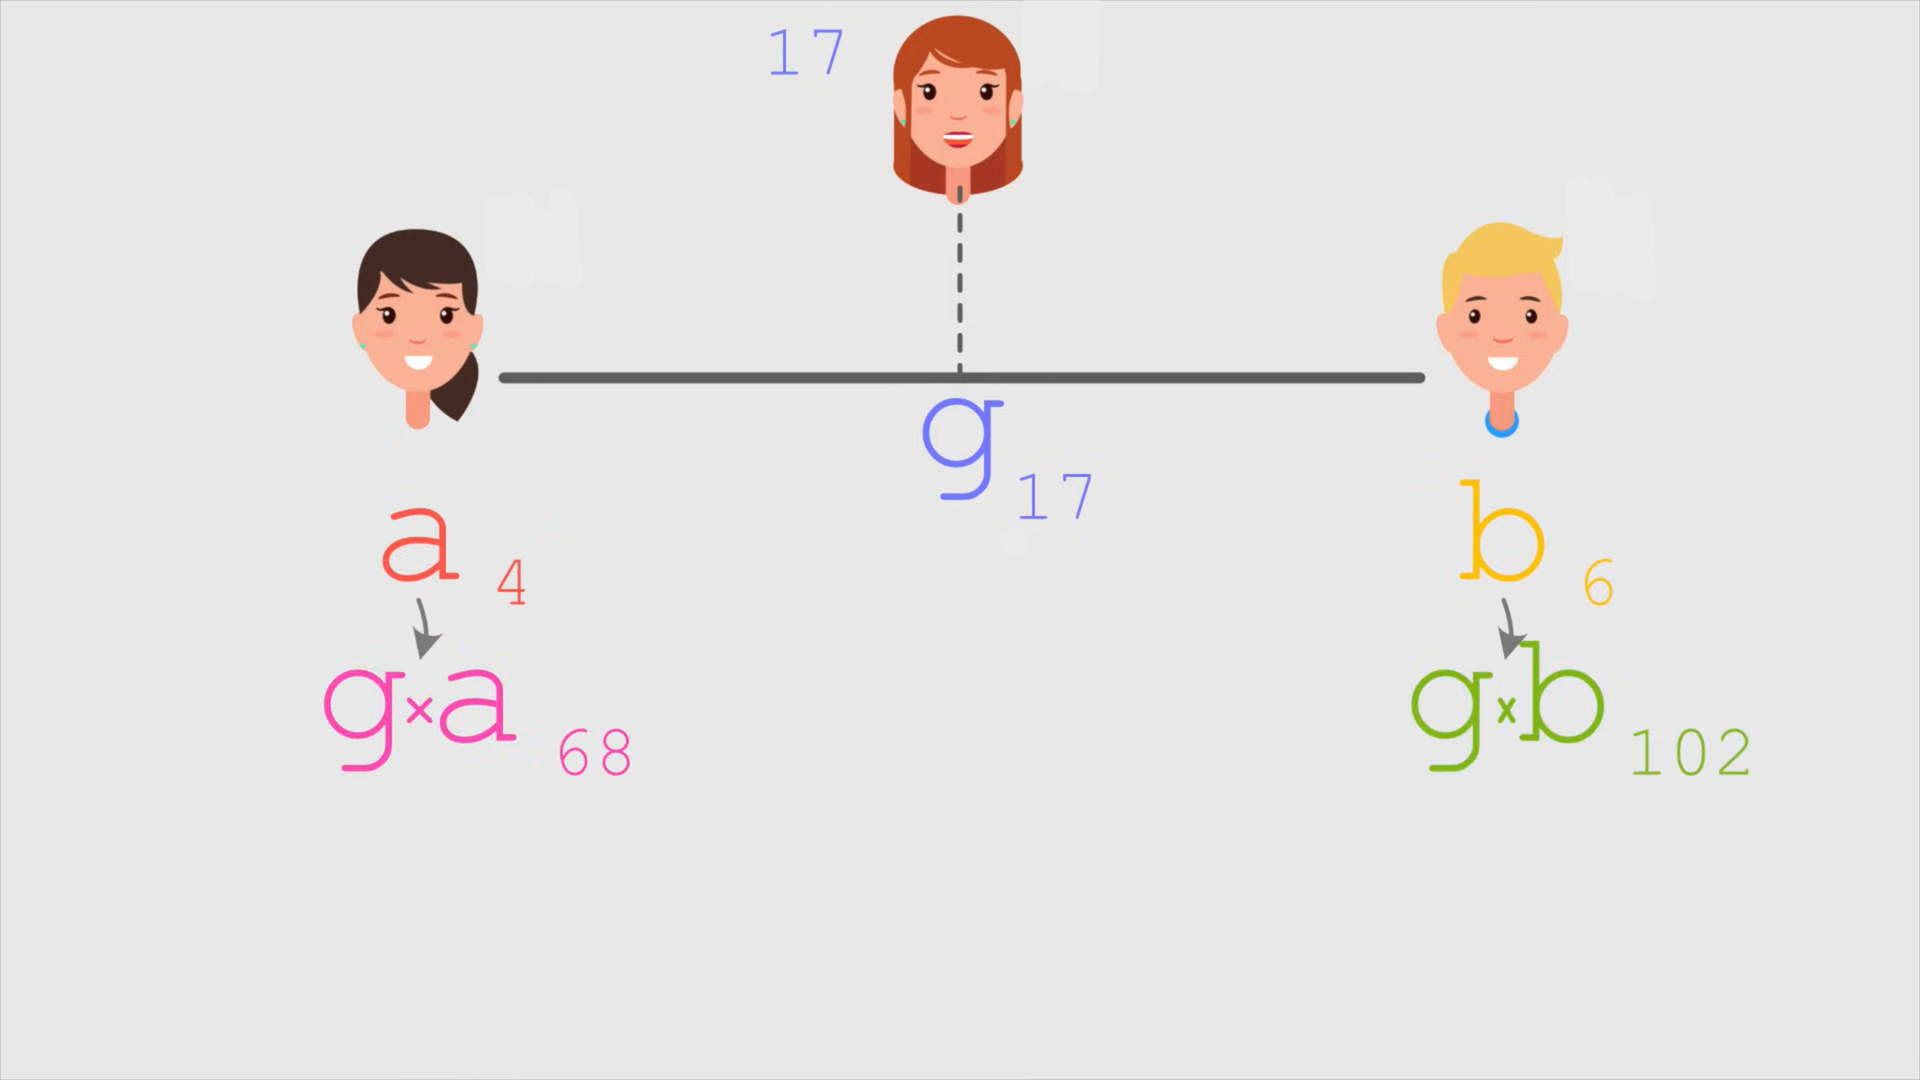
\includegraphics[width=\textwidth, height=0.9\textheight, keepaspectratio]{rsa 4.png}
\end{frame}

\begin{frame}{RSA}
    \centering
    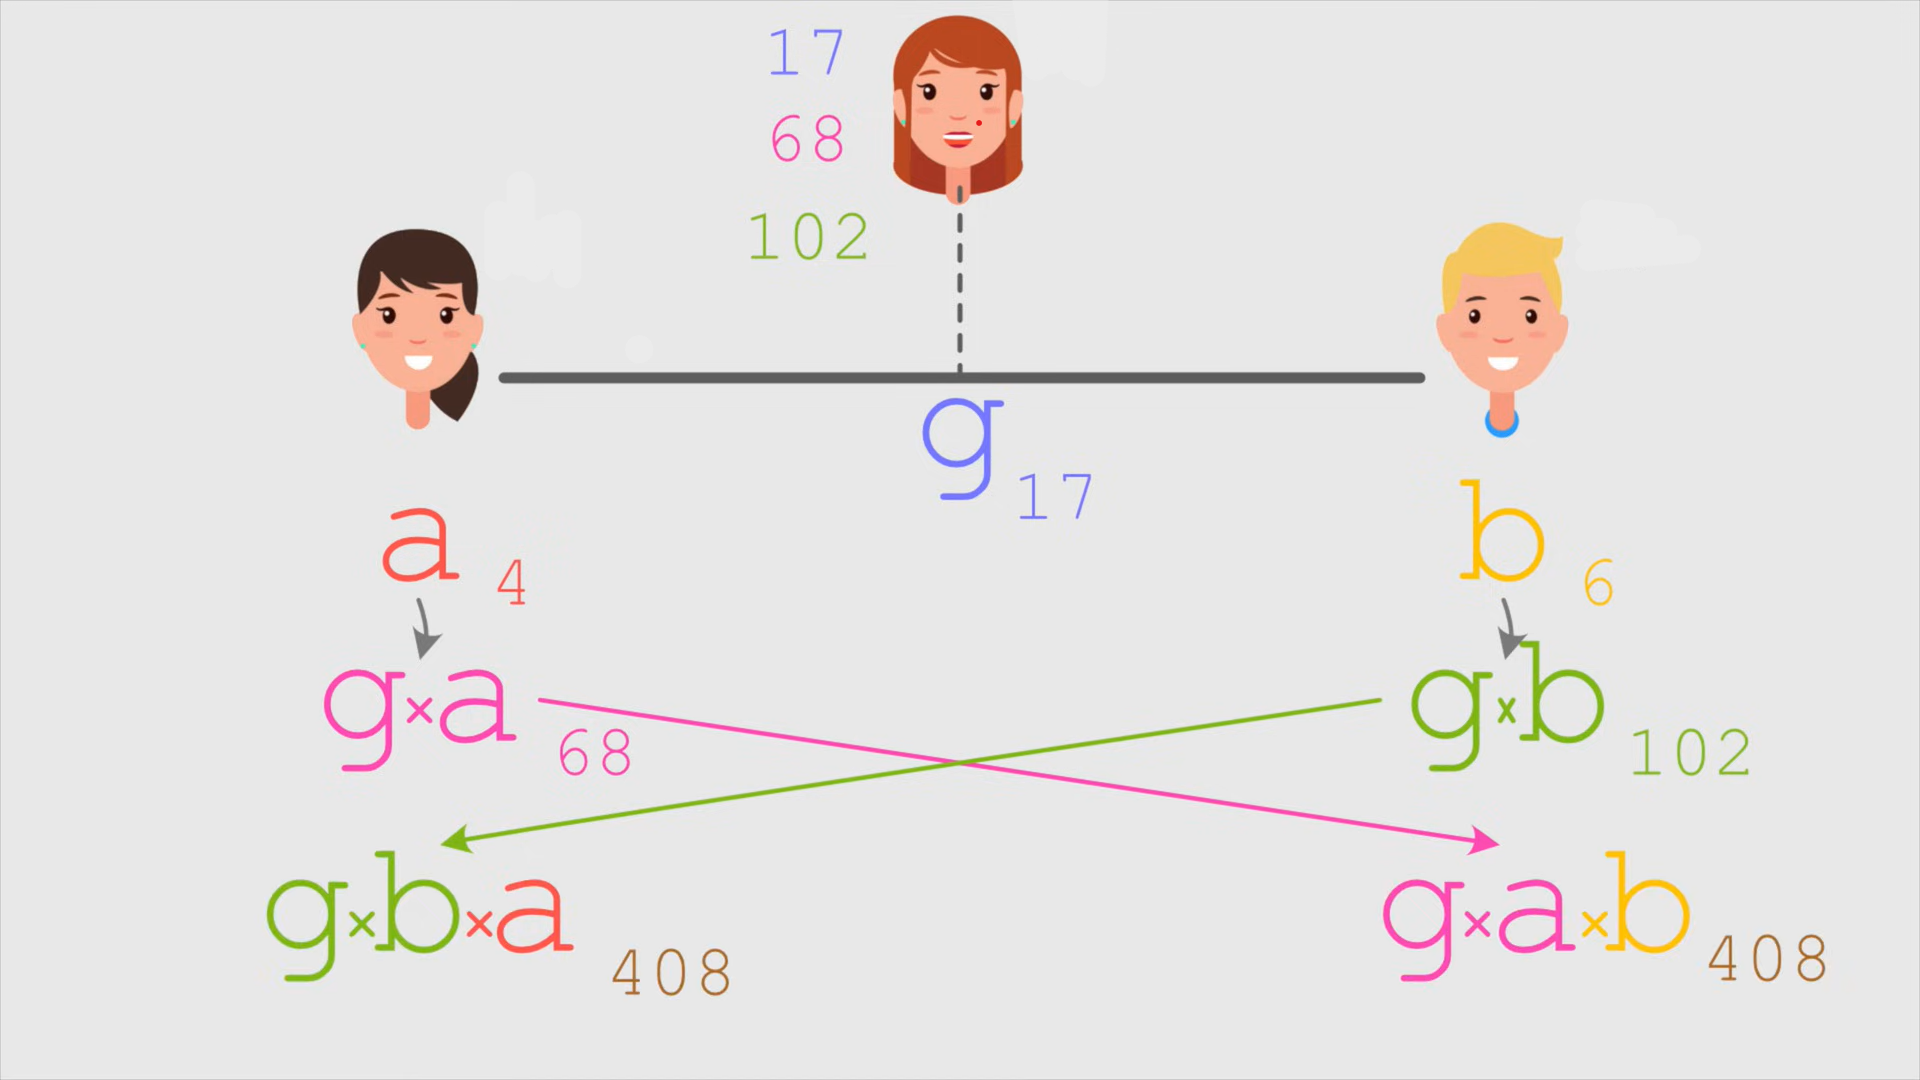
\includegraphics[width=\textwidth, height=0.9\textheight, keepaspectratio]{rsa 5.png}
\end{frame}

\begin{frame}{RSA}
    \centering
    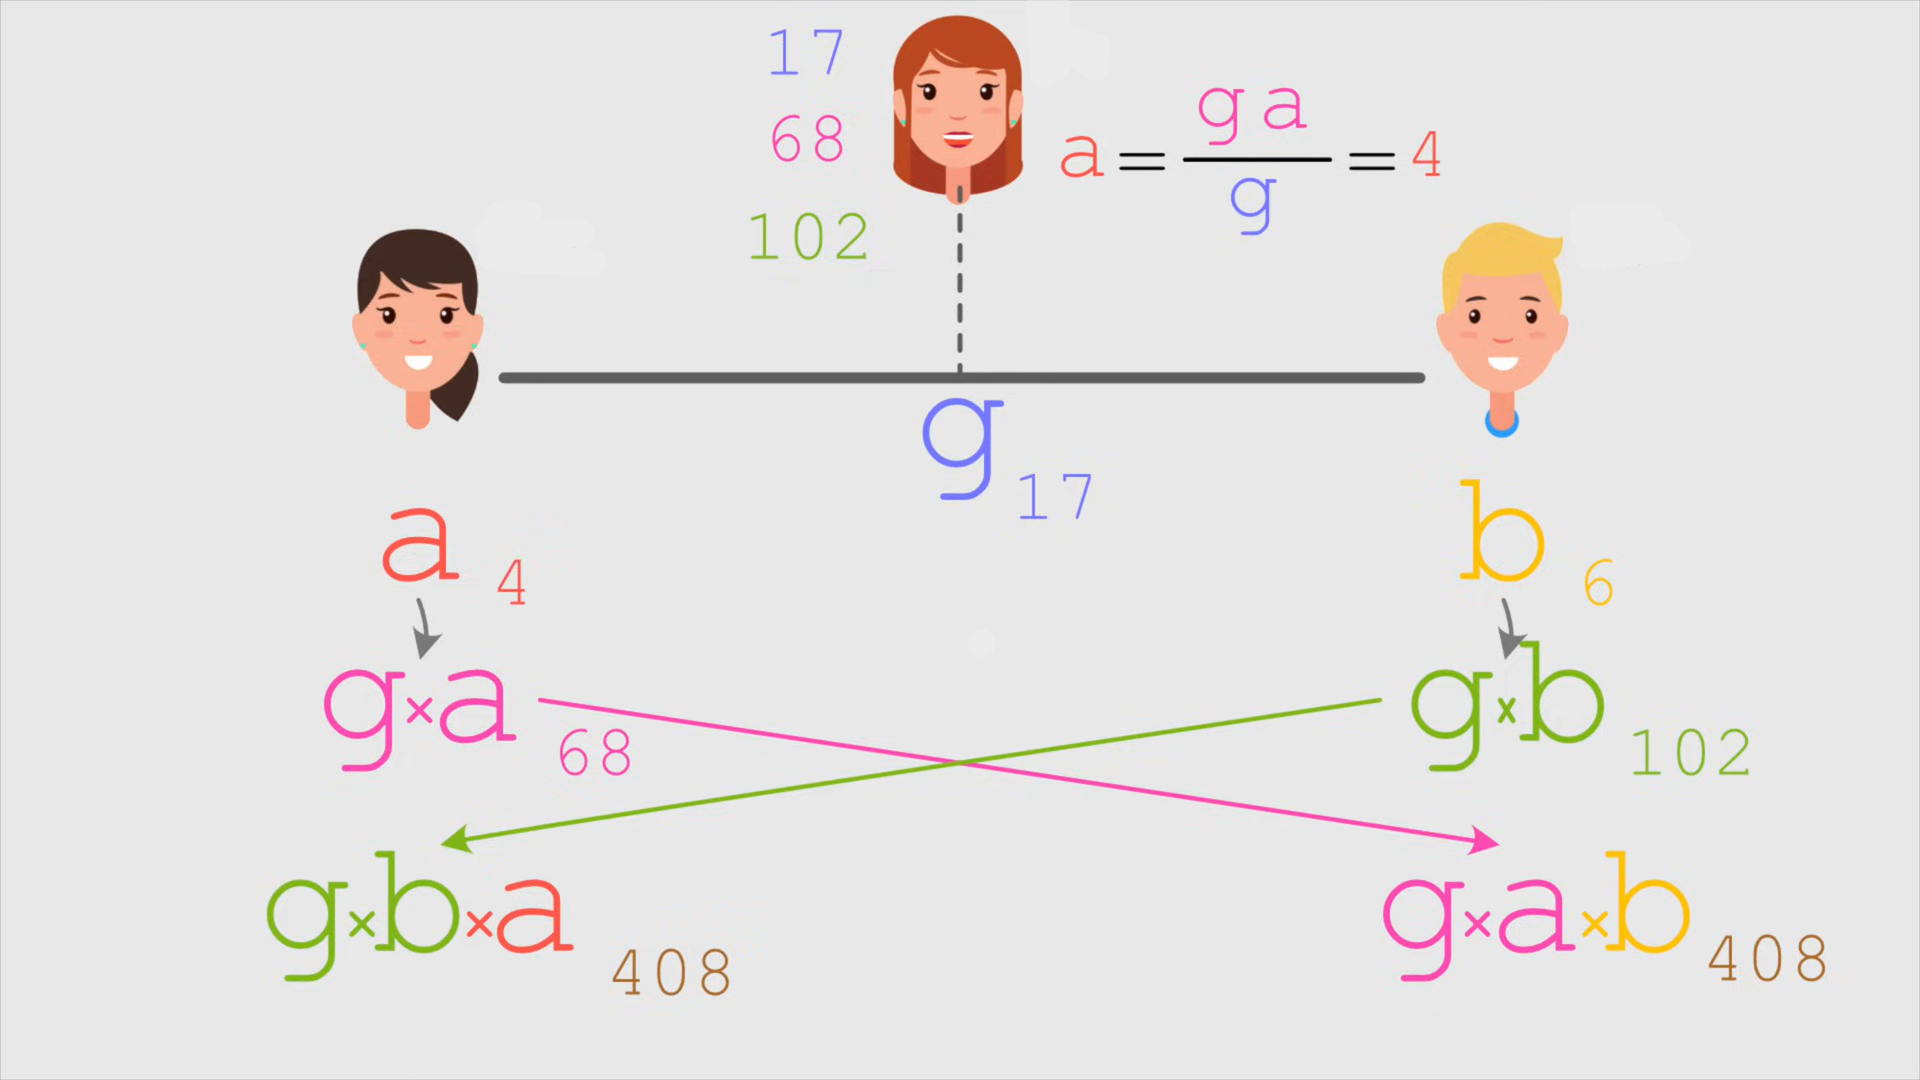
\includegraphics[width=\textwidth, height=0.9\textheight, keepaspectratio]{rsa 6.png}
\end{frame}

\begin{frame}{RSA}
    \centering
    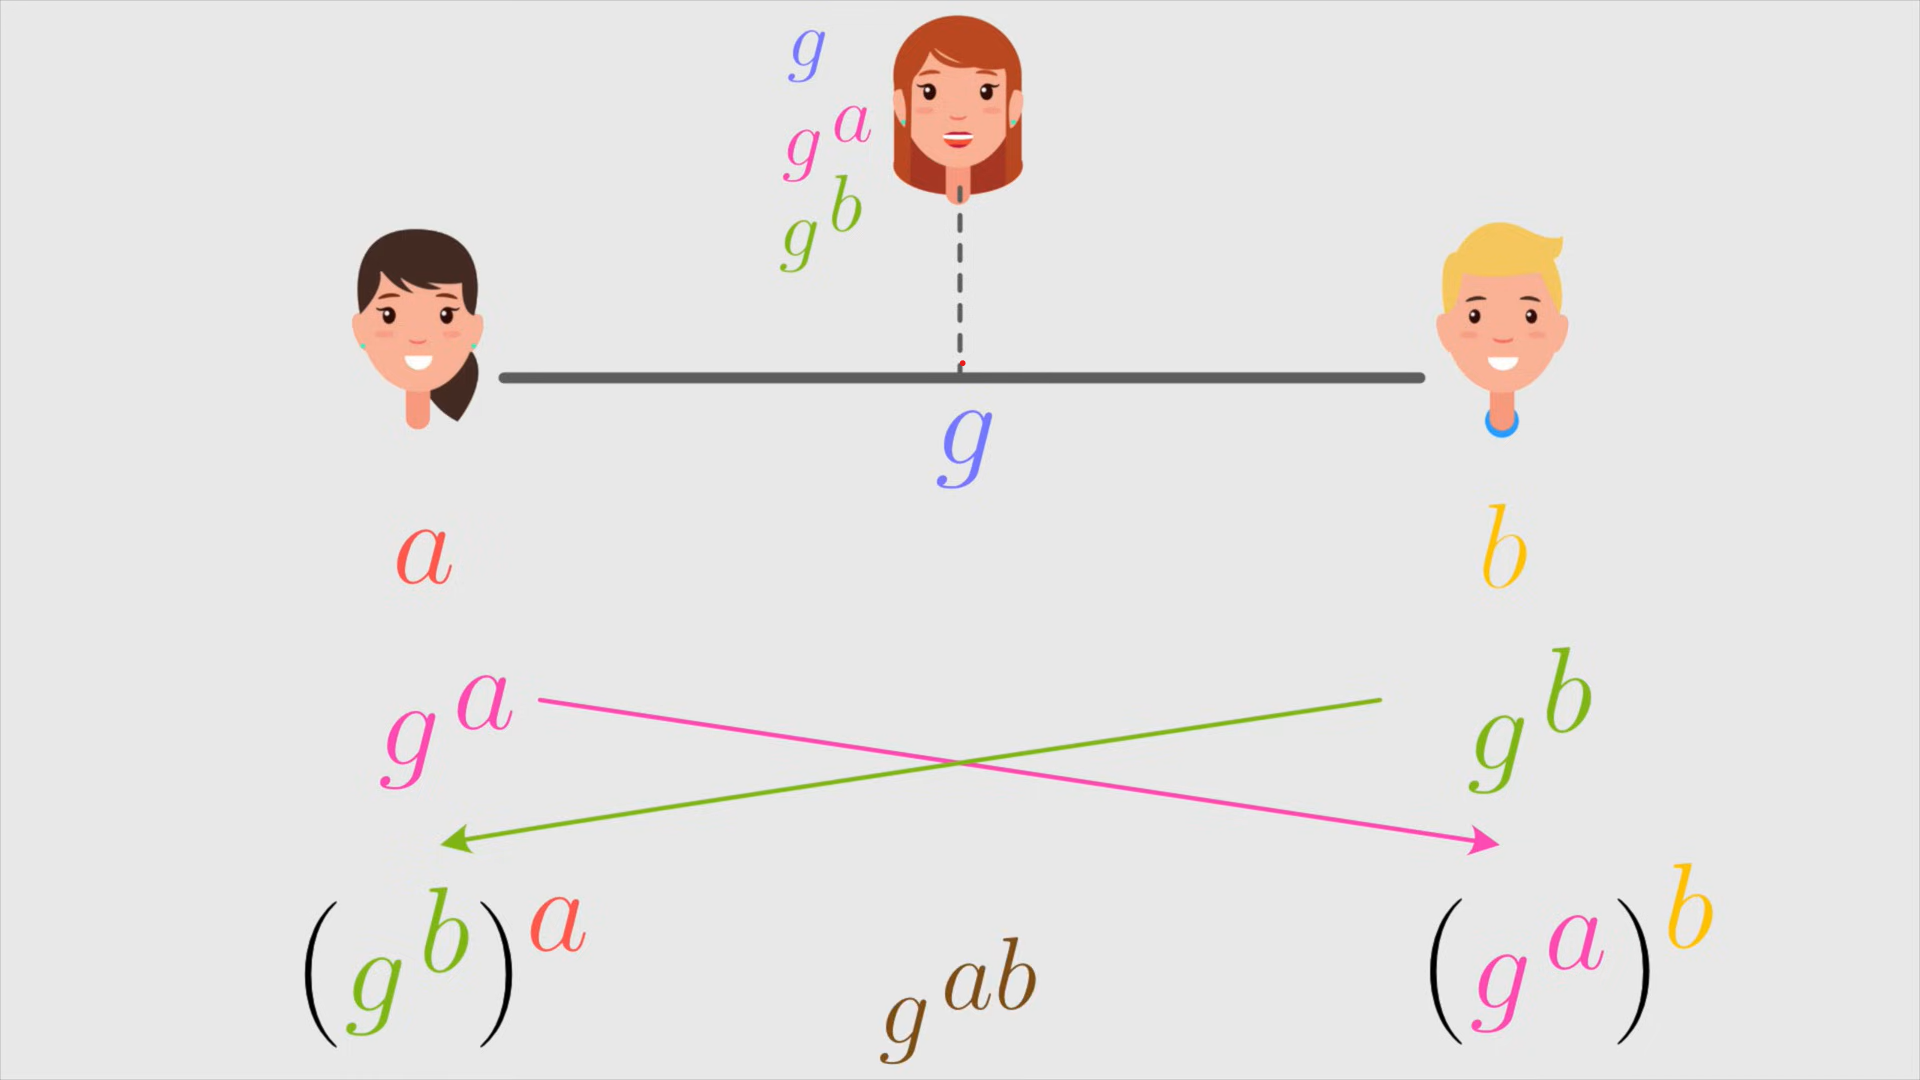
\includegraphics[width=\textwidth, height=0.9\textheight, keepaspectratio]{rsa 7.png}
\end{frame}

\begin{frame}{RSA}
    \centering
    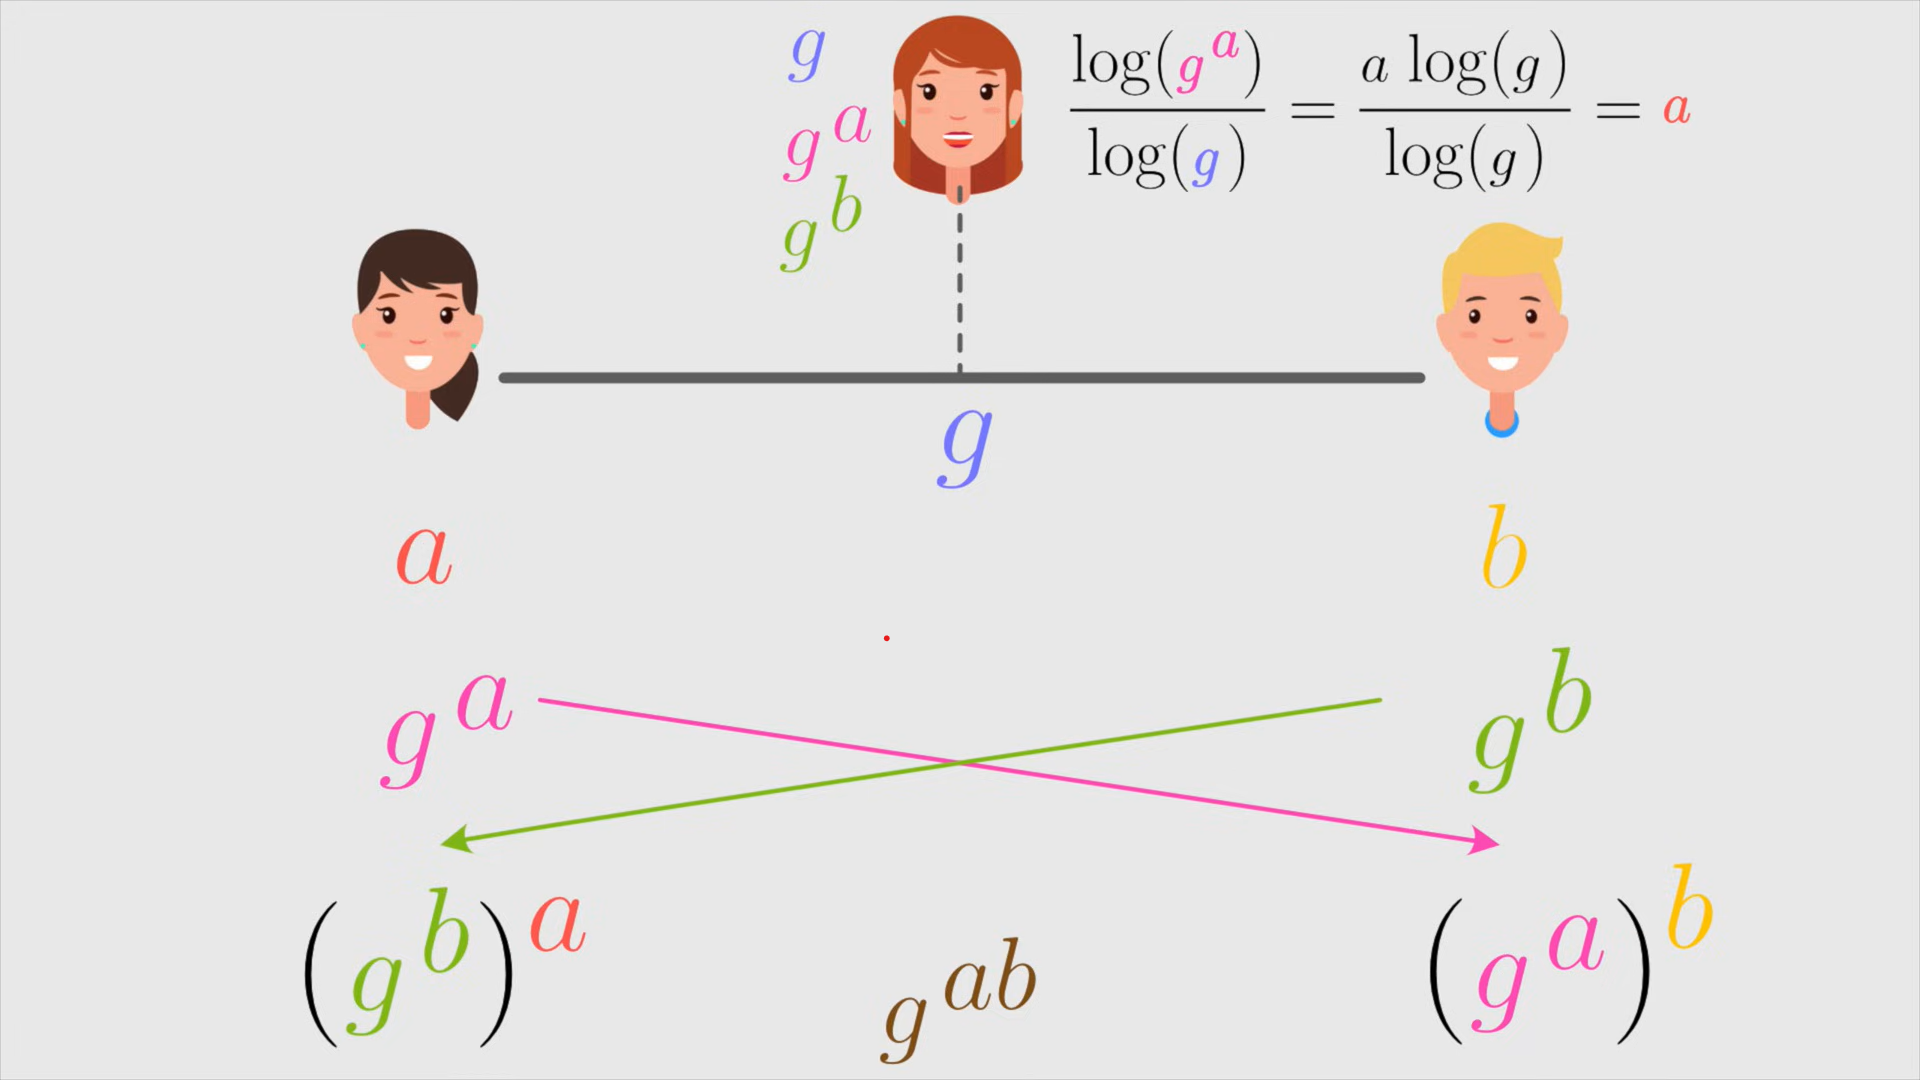
\includegraphics[width=\textwidth, height=0.9\textheight, keepaspectratio]{rsa 8.png}
\end{frame}

\begin{frame}{Reminder: Modulo and Diffie-Hellman}
    \begin{columns}
        \column{0.6\textwidth}
        \begin{block}{Understanding Modulo}
            The modulo operation finds the remainder when dividing one number by another.\\
            Example:
            \[
            17 \mod 3 = 2
            \]
            Because:
            \[
            17 = 5 \times 3 + 2
            \]
        \end{block}
       
        \column{0.4\textwidth}
        \centering
        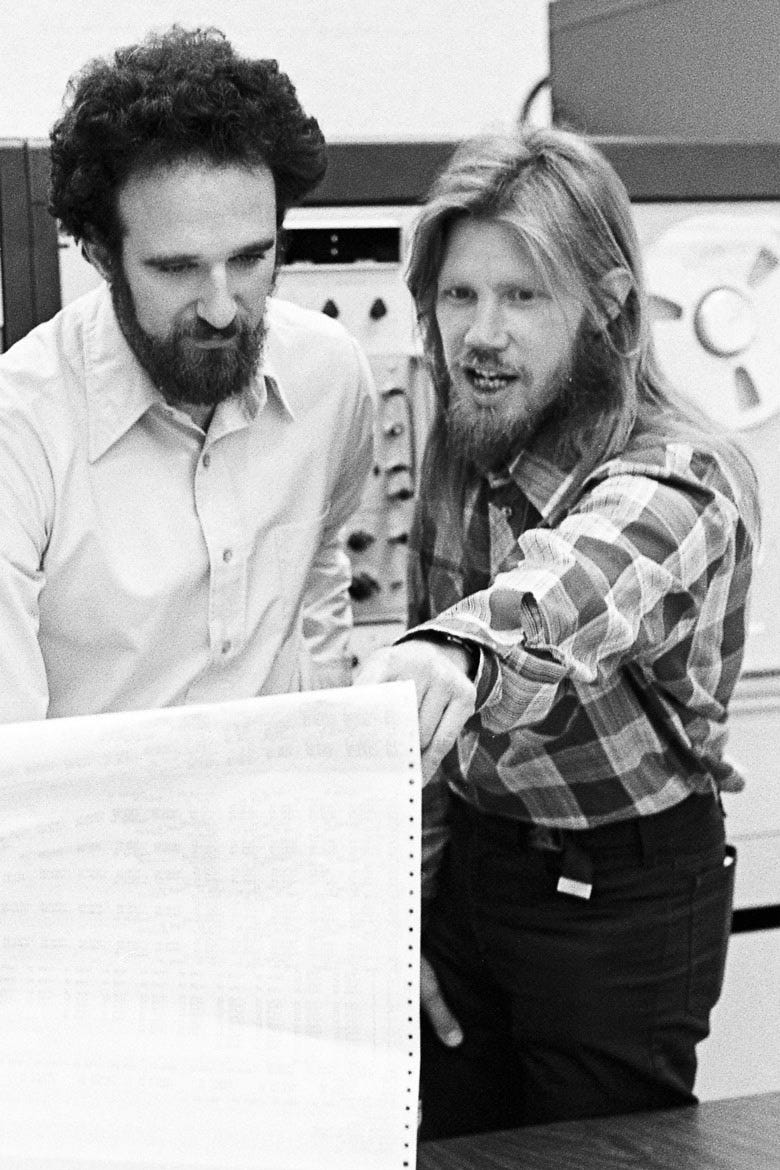
\includegraphics[width=0.9\textwidth]{diffiehellman.jpg}
    \end{columns}
\end{frame}


\begin{frame}{RSA}
    \centering
    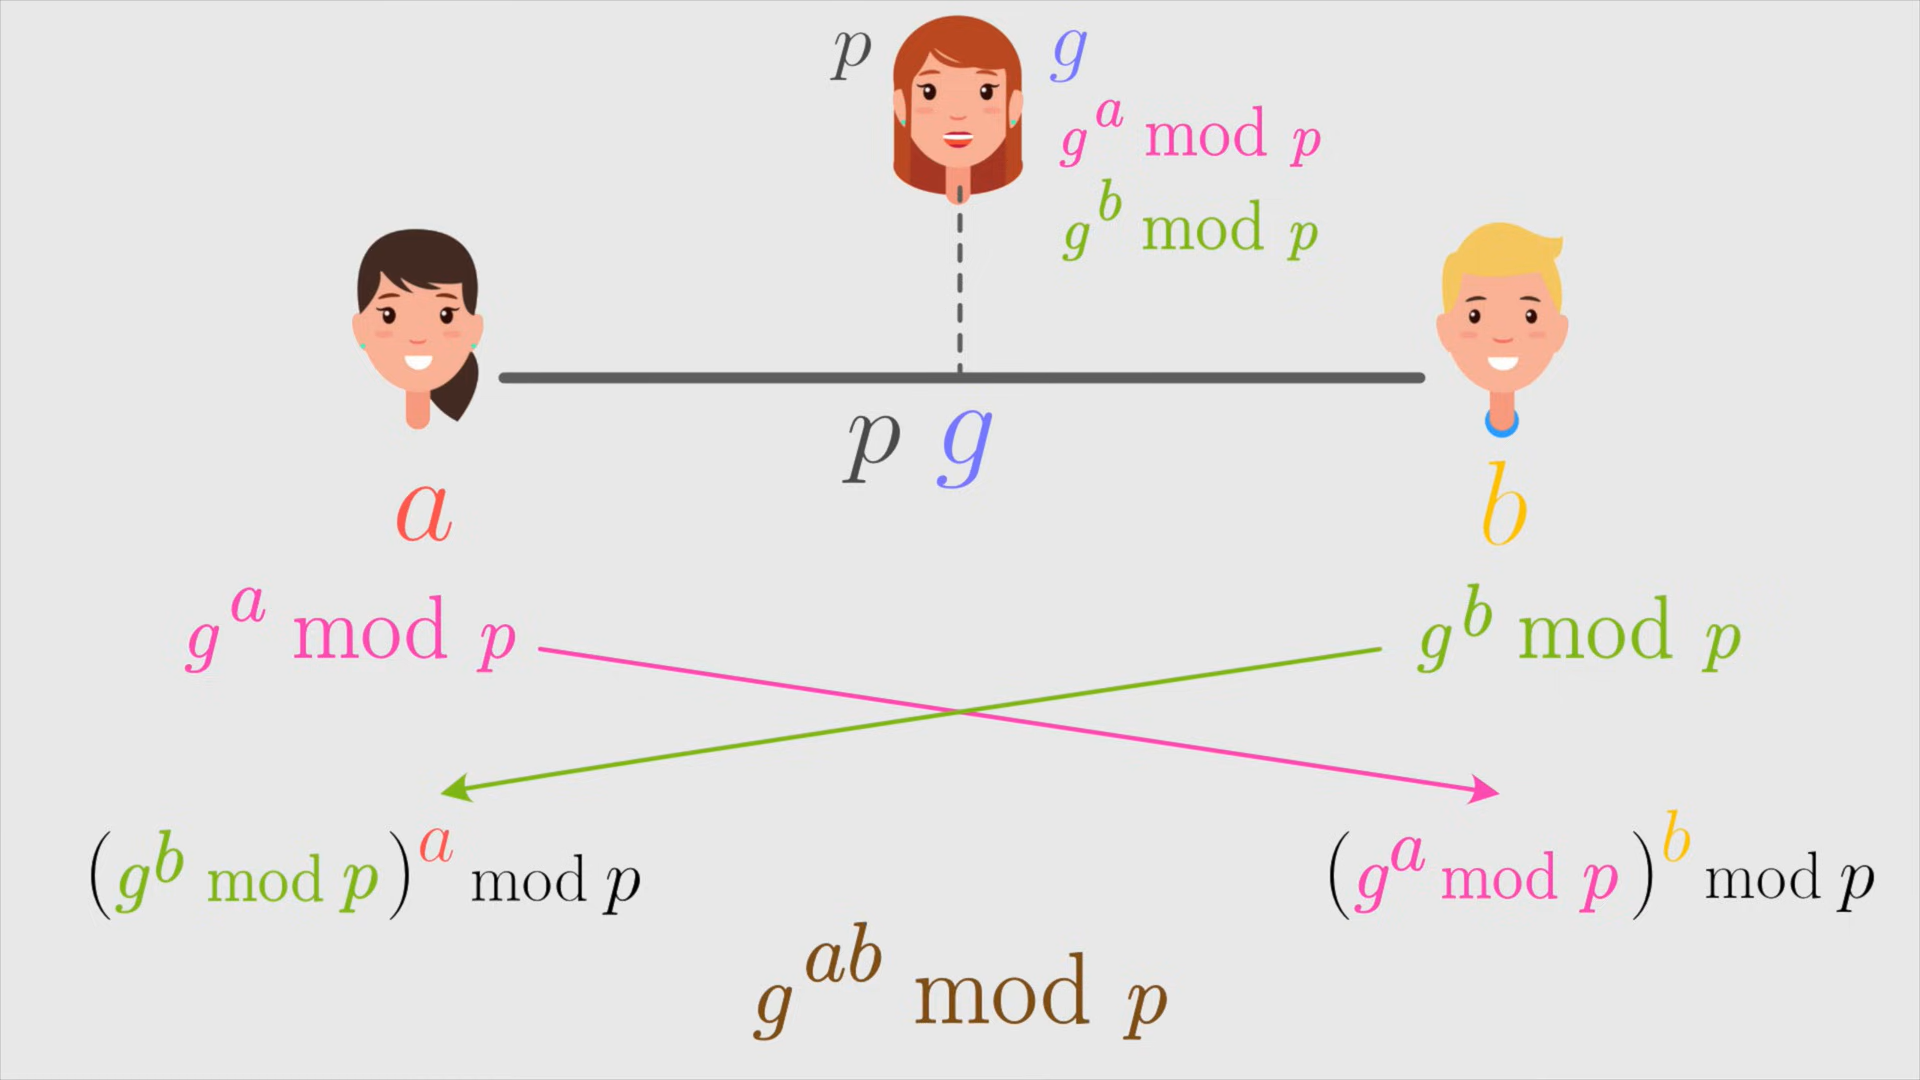
\includegraphics[width=\textwidth, height=0.9\textheight, keepaspectratio]{rsa 9.png}
\end{frame}

\begin{frame}{Security and Attacks}
    \centering
    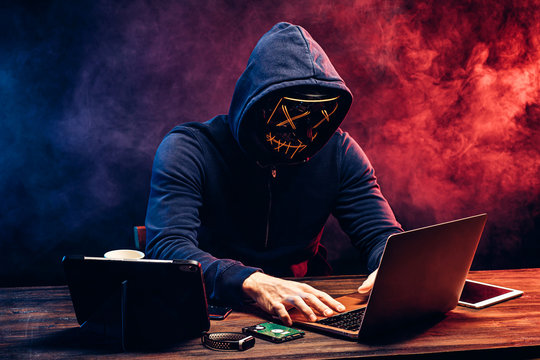
\includegraphics[width=\textwidth, height=0.9\textheight, keepaspectratio]{hacker.jpg}
\end{frame}


\section{Quantum computing}
\begin{frame}
  \frametitle{Outline}
  \tableofcontents[currentsection]
\end{frame}

\begin{frame}{Quantum computing}
	\centering
	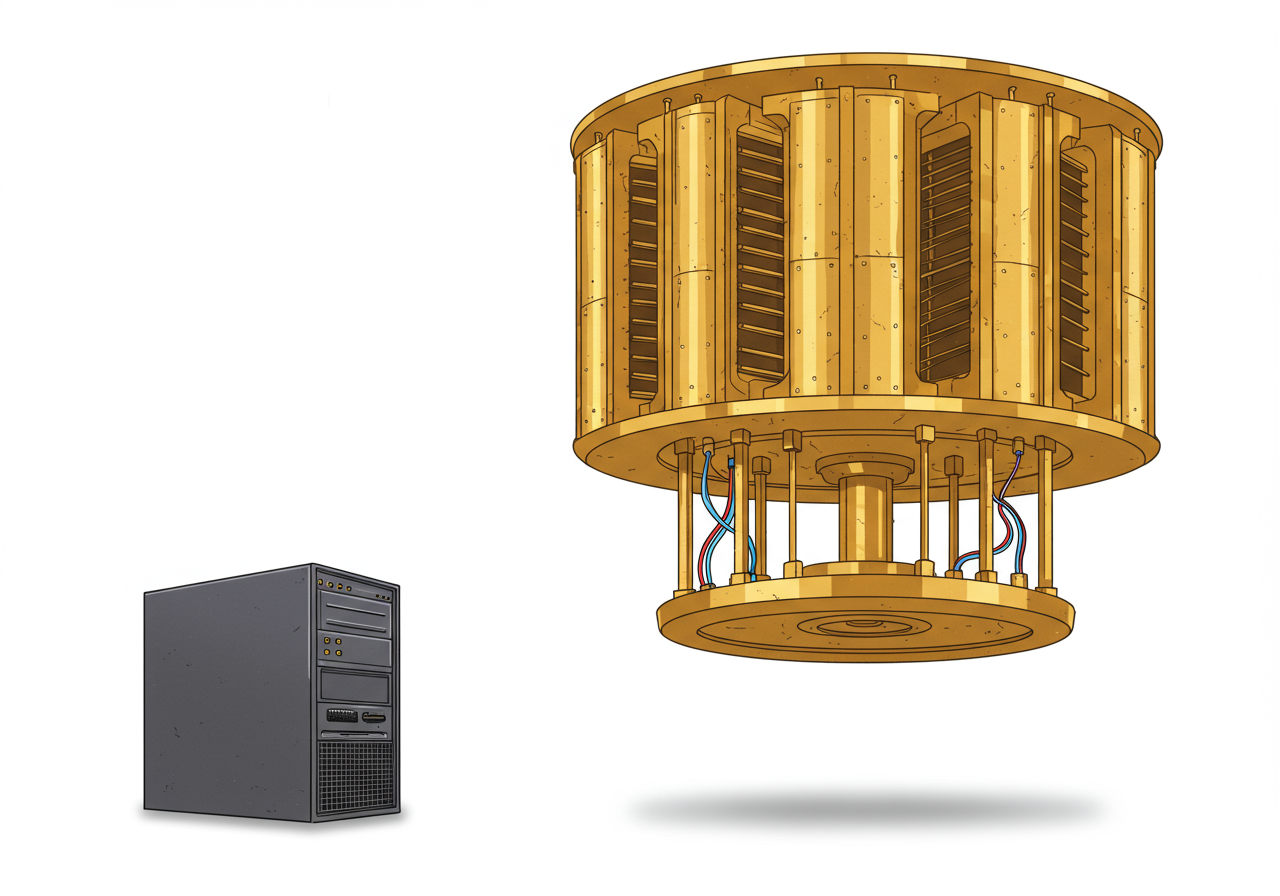
\includegraphics[width=0.8\textwidth]{classical-vs-quantum.png}
\end{frame}

\subsection{Introduction to the quantum world}
\begin{frame}
  \frametitle{Outline}
  \tableofcontents[currentsection,currentsubsection]
\end{frame}

\subsubsection*{Qubits}
\begin{frame}{Qubits}
\begin{linenumbers}
	\begin{block}<+->{Classical bit}
		$b \in \{0, 1\}$
		\begin{itemize}[<+->]
			\item $0$
			\item $1$
		\end{itemize}
	\end{block}

	\begin{block}<+->{Quantum bit}
		$\ket{\psi} \in \mathbb{C}^2$
		\begin{columns}[T,onlytextwidth]
			\column{0.5\textwidth}
				\begin{itemize}[<+->]
					\item $\ket{0} = \begin{bmatrix} 1 \\ 0 \end{bmatrix}$
					\item $\ket{1} = \begin{bmatrix} 0 \\ 1 \end{bmatrix}$
				\end{itemize}
			\column{0.5\textwidth}
				\begin{itemize}[<+->]
					\item $\ket{+} = \frac{1}{\sqrt{2}}\begin{bmatrix} 1 \\ 1 \end{bmatrix}$
					\item $\ket{-} = \frac{1}{\sqrt{2}}\begin{bmatrix} 1 \\ -1 \end{bmatrix}$
				\end{itemize}
		\end{columns}
	\end{block}
\end{linenumbers}
\end{frame}


\subsubsection*{Measurements}
\begin{frame}{Measurements}
	\begin{linenumbers}
		\begin{block}<+->{Why measuring ?}
			We cannot read superposition. When we look at a qubit, it collapses to a classical bit.
		\end{block}
		\begin{block}<+->{What do we get ?}
			We measure $0$ or $1$ with a probability that depends on the state of the qubit.
			\begin{columns}[T,onlytextwidth]
				\column{0.5\textwidth}
					\begin{itemize}[<+->]
						\item $\ket{0}$ $\rightarrow 0$ (100\%)
						\item $\ket{1}$ $\rightarrow 1$ (100\%)
					\end{itemize}
				\column{0.5\textwidth}
					\begin{itemize}[<+->]
						\item $\ket{+}$ $\rightarrow 0$ (50\%), $1$ (50\%)
					\item $\ket{-}$ $\rightarrow 0$ (50\%), $1$ (50\%)
					\end{itemize}
			\end{columns}
		\end{block}
	\end{linenumbers}
\end{frame}

\subsubsection*{Gates}
\begin{frame}{NOT gate}
\begin{linenumbers}
    \begin{block}<+->{X gate}
			\begin{itemize}
					\item $X\ket{0} \rightarrow \ket{1}$
					\item $X\ket{1} \rightarrow \ket{0}$
			\end{itemize}
		\end{block}
		\begin{block}<+->{Circuit representation}
			\centering
			\begin{quantikz}
				\lstick{$\ket{\psi}$} & \gate{X} & \meter{}
			\end{quantikz}
    \end{block}
\end{linenumbers}
\end{frame}

\begin{frame}{Hadamard gate}
	\begin{block}<+->{H gate}
			\begin{columns}[T,onlytextwidth]
				\column{0.5\textwidth}
					\begin{itemize}
						\item $H\ket{0} \rightarrow \ket{+}$
						\item $H\ket{1} \rightarrow \ket{-}$
					\end{itemize}
				\column{0.5\textwidth}<+->
					\begin{itemize}
						\item $H\ket{+} \rightarrow \ket{0}$
						\item $H\ket{-} \rightarrow \ket{1}$
					\end{itemize}
			\end{columns}
	\end{block}
	\begin{block}<+->{Circuit representation}
			\centering
			\begin{quantikz}
					\lstick{$\ket{\psi}$} & \gate{H} & \meter{}
			\end{quantikz}
	\end{block}
\end{frame}

\subsection{Quantum algorithms}
\begin{frame}
  \frametitle{Outline}
  \tableofcontents[currentsection,currentsubsection]
\end{frame}

\subsubsection*{Bernstein-Vazirani Problem}
\begin{frame}{Bernstein-Vazirani Problem}
\begin{linenumbers}
  \begin{block}<+->{Problem Definition}
    Given an oracle for a function $f$:
    \[ f : \{0, 1\}^n \rightarrow \{0, 1\} \]
    \[ f(\mathbf{x}) = \mathbf{x} \cdot \mathbf{s} \]
    where $\mathbf{s}$ is a secret bit string. Find $\mathbf{s}$ with the fewest oracle calls.  ($\cdot$ is the bitwise dot product, XOR sum).
  \end{block}
\end{linenumbers}
\end{frame}

\subsubsection*{Classical Algorithm}
\begin{frame}{Classical Algorithm - Example}
\begin{linenumbers}
  \begin{block}<+->{Example (n=2)}
    To find $\mathbf{s} = s_0s_1$:
    \begin{itemize}[<+->]
        \item Query $f(10) = 1 \cdot s_0 + 0 \cdot s_1 = s_0$
        \item Query $f(01) = 0 \cdot s_0 + 1 \cdot s_1 = s_1$
    \end{itemize}
    Requires 2 queries.
  \end{block}
\end{linenumbers}
\end{frame}

\begin{frame}{Classical Algorithm - General Case}
	\begin{linenumbers}
		\begin{block}<+->{Classical complexity: $\mathcal{O}(n)$}
			We need to isolate each bit of $\mathbf{s}$ by querying with inputs that have a single '1'. This requires $n$ queries for an $n$-bit string.
		\end{block}
	\end{linenumbers}
	\end{frame}
	

\subsubsection*{Quantum Algorithm}
\begin{frame}{Quantum Algorithm - Overview}
\begin{linenumbers}
	\begin{block}<+->{Quantum complexity: $\mathcal{O}(1)$}
		The quantum algorithm can find $\mathbf{s}$ with just \textbf{one} query.  It uses superposition to query all possible inputs simultaneously.
	\end{block}
\end{linenumbers}
\end{frame}

\begin{frame}{Quantum Algorithm - Circuit}
	\begin{linenumbers}
		\begin{block}<+->{Circuit Diagram}
			\centering
			\begin{quantikz}
				\lstick{} & \ket{0} & \gate{H} & \gate[2]{U_f} & \gate{H} & \meter{} & \qw \\
				\lstick{} & \ket{0} & \gate{H} &               & \gate{H} & \meter{} & \qw
				\end{quantikz}
		\end{block}
			\begin{block}<+->{Explanation}
			\begin{itemize}
					\item  $H$ : Hadamard gates on all $n$ input qubits (creates superposition).
					\item $U_f$ : The quantum oracle.
					\item Final Hadamards and measurement reveal $\mathbf{s}$.
			\end{itemize}
	\end{block}
	\end{linenumbers}
	\end{frame}

\subsubsection*{Breaking RSA}
\begin{frame}{Shor's Algorithm}
\begin{linenumbers}
  \begin{block}<+->{Complexity Gain}
        Classical factoring is very slow (roughly $\mathcal{O}(e^{\sqrt[3]{n}})$). Shor's algorithm is much faster (polynomial, $\mathcal{O}(n^3)$).
  \end{block}
    \begin{block}<+->{Requirements}
        \begin{itemize}[<+->]
            \item Requires a large number of high-quality (low-error) qubits (roughly $2n$ for an $n$-bit number).
            \item  We currently don't have quantum computers large and stable enough to break practical RSA encryption.
        \end{itemize}
    \end{block}
\end{linenumbers}
\end{frame}

\section{Post-Quantum cryptography}
\begin{frame}
  \frametitle{Outline}
  \tableofcontents[currentsection]
\end{frame}

\subsection{Intro to PQ cryptography}
\begin{frame}
  \frametitle{Outline}
  \tableofcontents[currentsection,currentsubsection]
\end{frame}

\begin{frame}{What is PQ cryptography}
	\begin{block}<+->{What it is:}
		\begin{itemize}
			\item Based on (other) mathematical problems
			\item Considered unsolvable by a quantum computer
			\item<+-> \textbf{And} by classical computers
		\end{itemize}
	\end{block}

	\begin{block}<+->{What it is not:}
		Cryptography \textbf{using} quantum technologies
		\begin{itemize}
			\item Many cases where it is unusable
			\item Deprecated from governmental institutions (NSA, ENISA\footnote{\url{doi.org/10.2824/92307}}, ANSSI)
		\end{itemize}
	\end{block}
\end{frame}

\begin{frame}{PQ cryptography now}
		
\includegraphics[width=0.1\textwidth]{NIST_logo.pdf}
		\centering
	\begin{block}{Standardization done by the NIST}
		\begin{itemize}
			\item 2016: Call for proposals for new standards
			\item 3 rounds of selection
			\item July 5, 2022: Announce of the first winners: 1 key encapsulation and 3 signatures protocols
			\item and a fourth round for PKE/KEM
			\item August 13, 2024: Specifications published
			\item March 11, 2025: Winner from the fourth round: 1 public key encryption
		\end{itemize}
	\end{block}

	Can be used in hybrid mode

	%i.e. With a pre-quantum protocol
\end{frame}

\begin{frame}{The PQ problems}
	\begin{block}{Families}
		\begin{itemize}
			\item Codes
			\item Hash functions % \footnote{Signature only}
			\item Isogenies
			\item Multivariates polynomials systems
			\item {\color<2>{red} Lattices}
%			\item Zero-knowledge proof\footnotemark[\value{footnote}]
		\end{itemize}
	\end{block}
\end{frame}

\begin{frame}{Why lattices ?}
	\begin{itemize}
		\item Well spread (One of the most studied)
		\item Good results
			\begin{table}[h!]
			\begin{tabular}{|c|c|}
				\hline
				\multicolumn{2}{|c|}{Encryption/Key encapsulation} \\
				\hline
				Crystals-Kyber & Lattices \\
				Hamming Quasi-Cyclic\footnote{From fourth round} & Codes \\
				\hline
				\multicolumn{2}{|c|}{Signatures} \\
				\hline
				Crystals-Dilithium & Lattices \\
				Falcon & Lattices \\
				Sphincs+ & Hash \\
				\hline
			\end{tabular}
			\center
			\caption{Results from the NIST}
			\end{table}
	\end{itemize}
\end{frame}

\subsection{Lattice-based cryptography}
\begin{frame}
  \frametitle{Outline}
  \tableofcontents[currentsection,currentsubsection]
\end{frame}

\subsubsection{What is a lattice ?}
\begin{frame}{Some definitions}
	\begin{block}<+->{The unformal definition}
		A arrangement of points in space, following a regular pattern
	\end{block}
	% TODO : Examples
	\begin{figure}[H]
		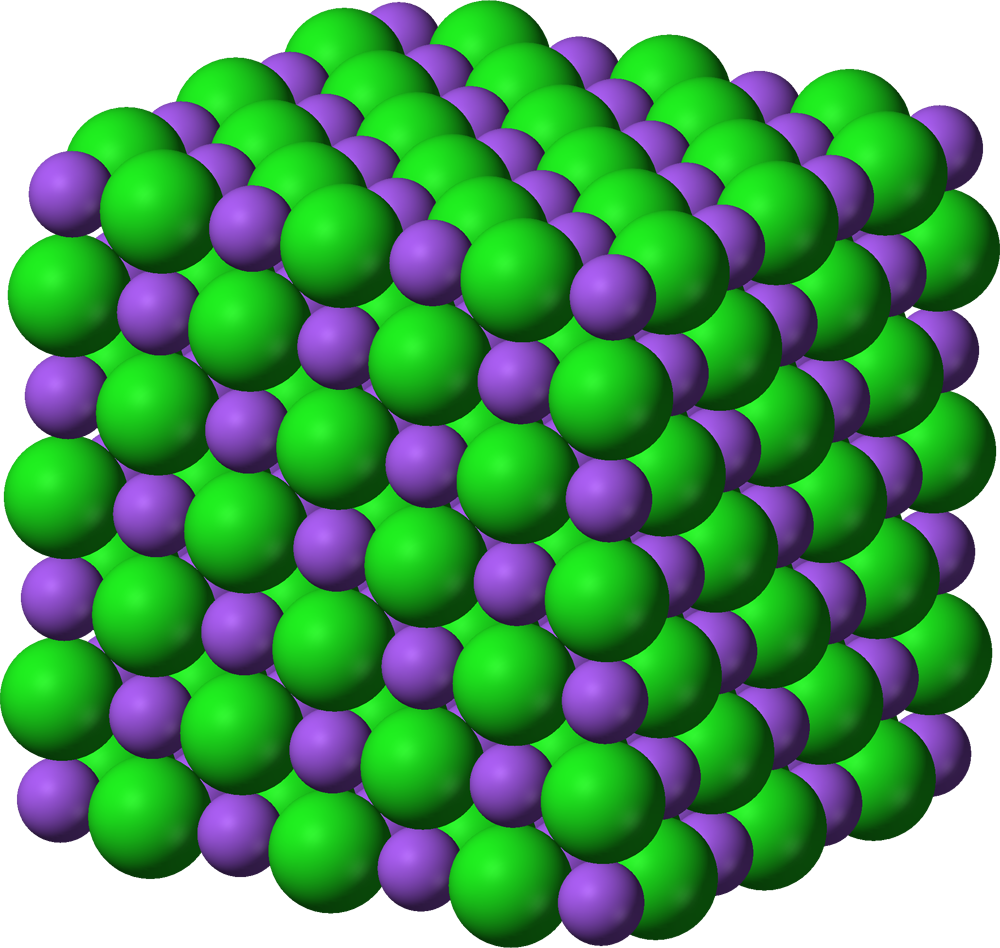
\includegraphics[width=0.2\textwidth]{Sodium-chloride-3D-ionic.png}
		\center
		\caption{Crystal structure of NaCl}
	\end{figure}

	\begin{block}<+->{The (more) formal one}
		A discret subgroup of $\mathbb{R}^n$, with the euclidean distance
	\end{block}
	\begin{itemize}
		\item[$\Rightarrow$]<+-> We have vectors, dot/scalar product and matrices
	\end{itemize}
\end{frame}

\begin{frame}{Example}
	% \begin{columns}[t]
	% \begin {column}{0.5\textwidth}
	\begin{figure}
		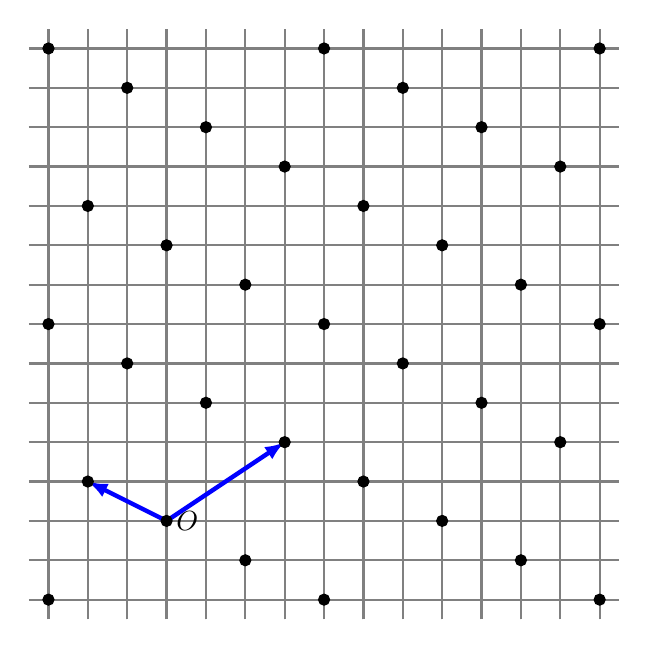
\begin{tikzpicture}
		\foreach \i in {1, ..., 8, 1.5, ..., 7.5} {
			\draw [gray, thick] (\i, 0.75) -- (\i, 8.25);
		}
		\foreach \i in {1, ..., 8, 1.5, ..., 7.5} {
			\draw [gray, thick] (0.75, \i) -- (8.25, \i);
		}

		%%% Basis
		\draw[ultra thick, blue, arrows={-{Latex[length=2.5mm]}}] (2.5, 2) -- (4, 3);
		\draw[ultra thick, blue, arrows={-{Latex[length=2.5mm]}}] (2.5, 2) -- (1.5, 2.5);

		%%% The lattice's points
		\filldraw[black] (8, 1) circle (2pt);

		\filldraw[black] (7, 1.5) circle (2pt);

		\filldraw[black] (4.5, 1) circle (2pt);
		\filldraw[black] (6, 2) circle (2pt); % end
		\filldraw[black] (7.5, 3) circle (2pt);

		\filldraw[black] (3.5, 1.5) circle (2pt);
		\filldraw[black] (5, 2.5) circle (2pt);
		\filldraw[black] (6.5, 3.5) circle (2pt); % end
		\filldraw[black] (8, 4.5) circle (2pt);

		\filldraw[black] (1, 1) circle (2pt); % beg
		\filldraw[black] (2.5, 2) circle (2pt) node[anchor=west]{$O$};
		\filldraw[black] (4, 3) circle (2pt);
		\filldraw[black] (5.5, 4) circle (2pt);
		\filldraw[black] (7, 5) circle (2pt); % end

		\filldraw[black] (1.5, 2.5) circle (2pt); % beg
		\filldraw[black] (3, 3.5) circle (2pt);
		\filldraw[black] (4.5, 4.5) circle (2pt);
		\filldraw[black] (6, 5.5) circle (2pt);
		\filldraw[black] (7.5, 6.5) circle (2pt); % end

		\filldraw[black] (2, 4) circle (2pt); % beg
		\filldraw[black] (3.5, 5) circle (2pt);
		\filldraw[black] (5, 6) circle (2pt);
		\filldraw[black] (6.5, 7) circle (2pt);
		\filldraw[black] (8, 8) circle (2pt); % end

		\filldraw[black] (1, 4.5) circle (2pt);
		\filldraw[black] (2.5, 5.5) circle (2pt); % beg
		\filldraw[black] (4, 6.5) circle (2pt);
		\filldraw[black] (5.5, 7.5) circle (2pt);

		\filldraw[black] (1.5, 6) circle (2pt);
		\filldraw[black] (3, 7) circle (2pt);  % beg
		\filldraw[black] (4.5, 8) circle (2pt);

		\filldraw[black] (2, 7.5) circle (2pt);

		\filldraw[black] (1, 8) circle(2pt);
		\end{tikzpicture}
		\center
	\end{figure}
	% \end{column}
	% \begin{column}{0.45\textwidth}
	% 	FIXME : Basis:

	% 	\[\left\{\left(\begin{matrix}3\\2\end{matrix}\right), \left(\begin{matrix}-2\\1\end{matrix}\right)\right\}\]
	% \end{column}
	% \end{columns}
\end{frame}

\begin{frame}{Learning with error problem}
	\begin{block}{One equation}
		For\begin{itemize}
			\item a secret vector $s$,
			\item a public one $a$,
			\item a small error $e$ and
			\item a public result $b$
		\end{itemize} solve $ a \cdot s + e = b$
	\end{block}
	% sk = (6, 5, 6, 2)
	% LWE:
	% [ 9  5  7 10] . sk + 11 = 9
	% [ 7 10  5  3] . sk + 12 = 10
	% [ 4  7  6  7] . sk + 1 = 6
	% [ 7  8  3 11] . sk + 0 = 5
	% [ 2  2 11  1] . sk + 1 = 0
	% [ 2  9  9  1] . sk + 0 = 9
	% S = (0, 0, 1, 0, 0, 1)
	% c = ((6, 3, 2, 8), 2)
	% x = 1
	% m = 0
	\pause
	Example in $\mathbb{Z}/13\mathbb{Z}$
	\[
		\left[\begin{matrix}
			9 & 5 & 7 & 10 \\
			7 & 10 & 5 & 3 \\
			4 & 7 & 6 & 7 \\
			7 & 8 & 3 & 11 \\
			2 & 2 & 11 & 1 \\
			2 & 9 & 9 & 1 \\
		\end{matrix}\right]
		\times
		\left[\begin{matrix}
			6 \\ 5 \\ 6 \\ 2
		\end{matrix}\right]
		+
		\left[\begin{matrix} -1 \\ -1 \\ 1 \\ 0 \\ 1 \\ 0 \end{matrix}\right]
		=
		\left[\begin{matrix} 10 \\ 10 \\ 6 \\ 5 \\ 0 \\ 9 \end{matrix}\right]
	\]
\end{frame}

\begin{frame}{Regev's algorithm}
	\begin{algorithm}[H]
		\caption{Encryption}\label{algo:regev_enc}
		\begin{algorithmic}
			\Require $M\in\{0, 1\}$, $m$ equations $a_i \cdot s + e_i = b_i$
			\State Choose $Sel\subseteq[\![0, m-1]\!]$ randomly
			\State $c_1 \gets \displaystyle\sum_{i\in Sel} a_i$
			\State $c_2 \gets \left(\displaystyle\sum_{i\in Sel} b_i\right) + M \times \floor{\frac{q}{2}}$
			\State \Return $(c_1, c_2)$
		\end{algorithmic}
	\end{algorithm}
		$M = 1$, $Sel = \{2, 5\}$
		\begin{align*}
			(4, 7, 6, 7), &\ 6 \\
			+ (2, 9, 9, 1), &\ 9 \\
			= (6, 3, 2, 8), &\ 2 + 1 \times 6 = 8
		\end{align*}
\end{frame}

\begin{frame}{Regev's algorithm (cont'd)}
	\begin{algorithm}[H]
		\caption{Decryption}\label{algo:regev_dec}
		\begin{algorithmic}
			\State $x \gets c_2 - c_1 \cdot s = \left(\displaystyle\sum_{i\in Sel} e_i\right) + M\times\floor{\frac{q}{2}}$ % \left(\displaystyle\sum_{i\in S} a_i \cdot s\right) + M\cdot\frac{q}{2} = M\cdot\frac{q}{2}$
			\If{$x\in \left[\floor{\frac{q}{4}}, \floor{\frac{3q}{4}} - 1\right]$}
				\State \Return 1
			\Else
				\State \Return 0
			\EndIf
		\end{algorithmic}
	\end{algorithm}
	\begin{itemize}
		\item $8 - (6, 3, 2, 8) \cdot (6, 5, 6, 2) = 8 - 1 = 7$
		\item $7 \in [3, 8] \rightarrow 1$
	\end{itemize}
\end{frame}

\begin{frame}{(Fully) homomorphic encryption}
	\begin{itemize}
		\item We can evaluate a circuit on encrypted data
		\item<2-> Two operations: $+$ and $\cdot$ (or $\times$)
		\item<2-> Obtained by transforming the function to apply with a compiler%\footnote{\url{https://heir.dev/}}
	\end{itemize}
	\begin{block}<3->{$eval$}
		For a function $f : P \times P \rightarrow P$ and encrypted data $C_1$ and $C_2$:
		\[eval(f, C_1, C_2) = Enc(f(Dec(C_1), Dec(C_2)))\]
	\end{block}
	\begin{itemize}
		\item<4-> Used to manipulate private data (e.g. Medical data, data science, Machine learning)
		\item<5-> Based on lattices (variant of LWE problem)
	\end{itemize}
\end{frame}

% subsection{Limits of PQ cryptography}
% begin{frame}
%  \frametitle{Outline}
%  \tableofcontents[currentsection,currentsubsection]
% end{frame}
% begin{frame}{Sizes of the keys and data}
%    \begin{tabular}{|c|c|}
%    	\hline
%    	TODO & \\
%    	\hline
%    \end{tabular}
% end{frame}
% 
% begin{frame}{Not necessarly robust to classical computer}
%    \begin{itemize}
%    	\item Example : Supersingular isogenies Diffie-Hellman key exchange
%    \end{itemize}
% end{frame}

\section{Conclusion}
\begin{frame}
  \frametitle{Outline}
  \tableofcontents[currentsection]
\end{frame}
\begin{frame}{Conclusion}
\begin{linenumbers}
    \begin{block}<+->{Summary of Key Points}
        \begin{itemize}
            \item Cryptography has evolved from simple secret writing to complex mathematical protocols.
            \item Quantum computing poses a significant threat to classical cryptographic schemes, particularly RSA.
            \item Post-Quantum cryptography offers potential solutions through lattice-based and other hard mathematical problems.
        \end{itemize}
    \end{block}
    
    \begin{block}<+->{Challenges and Future Perspectives}
        \begin{itemize}
            \item Quantum computers are not yet powerful enough to break RSA in practice, but research is advancing rapidly.
            \item Post-Quantum cryptography must balance security, efficiency, and scalability.
            \item The transition to quantum-safe cryptography is crucial for securing future communications.
        \end{itemize}
    \end{block}
    
\end{linenumbers}
\end{frame}

\end{document}
